% =================== Lesson 9: Citations and Bibliography ===================
\documentclass{article}
\begin{document}

According to \cite{tayab25} this has been happened....

\begin{thebibliography}{10}
    \bibitem{tayab25}
    Tayab. F, (25). Malware Detection using LLM
\end{thebibliography}

\end{document}

% \documentclass{article}
% \begin{document}

% According to \cite{tayab25} subtle increase in App development leads fast
% advancment in Mobile App usage!

% \begin{thebibliography}{10}
%     \bibitem{tayab25}
%     Tayab, F. (2025). Malware Detection System
%     \bibitem{tayab25}
%     Tayab, F. (2025). Malware Detection System

% \end{thebibliography}

% \end{document}

% =================== Lesson 8: Creating Tables ===================
% \documentclass{article}              % Define document type

% \begin{document}                     % Start document content

% \begin{table}[h]                     % Create table, position "here"
%     \centering                       % Center the table
%     \begin{tabular}{|c|c|c|}        % 3 centered columns with borders
%         \hline                       % Horizontal line
%         Name & Age & City \\         % Header row, & separates columns
%         \hline                       % Line under header
%         John & 25  & NYC  \\        % Data row 1
%         Jane & 30  & LA   \\        % Data row 2
%         \hline                       % Bottom border
%     \end{tabular}
%     \caption{Sample table}          % Table caption/title
% \end{table}

% \end{document}                       % End document

% =================== Lesson 7: Adding Images ===================
% \documentclass{article}
% \usepackage{graphicx}

% \begin{document}
% \section{My Figure}

% \begin{figure}
%     \centering
%     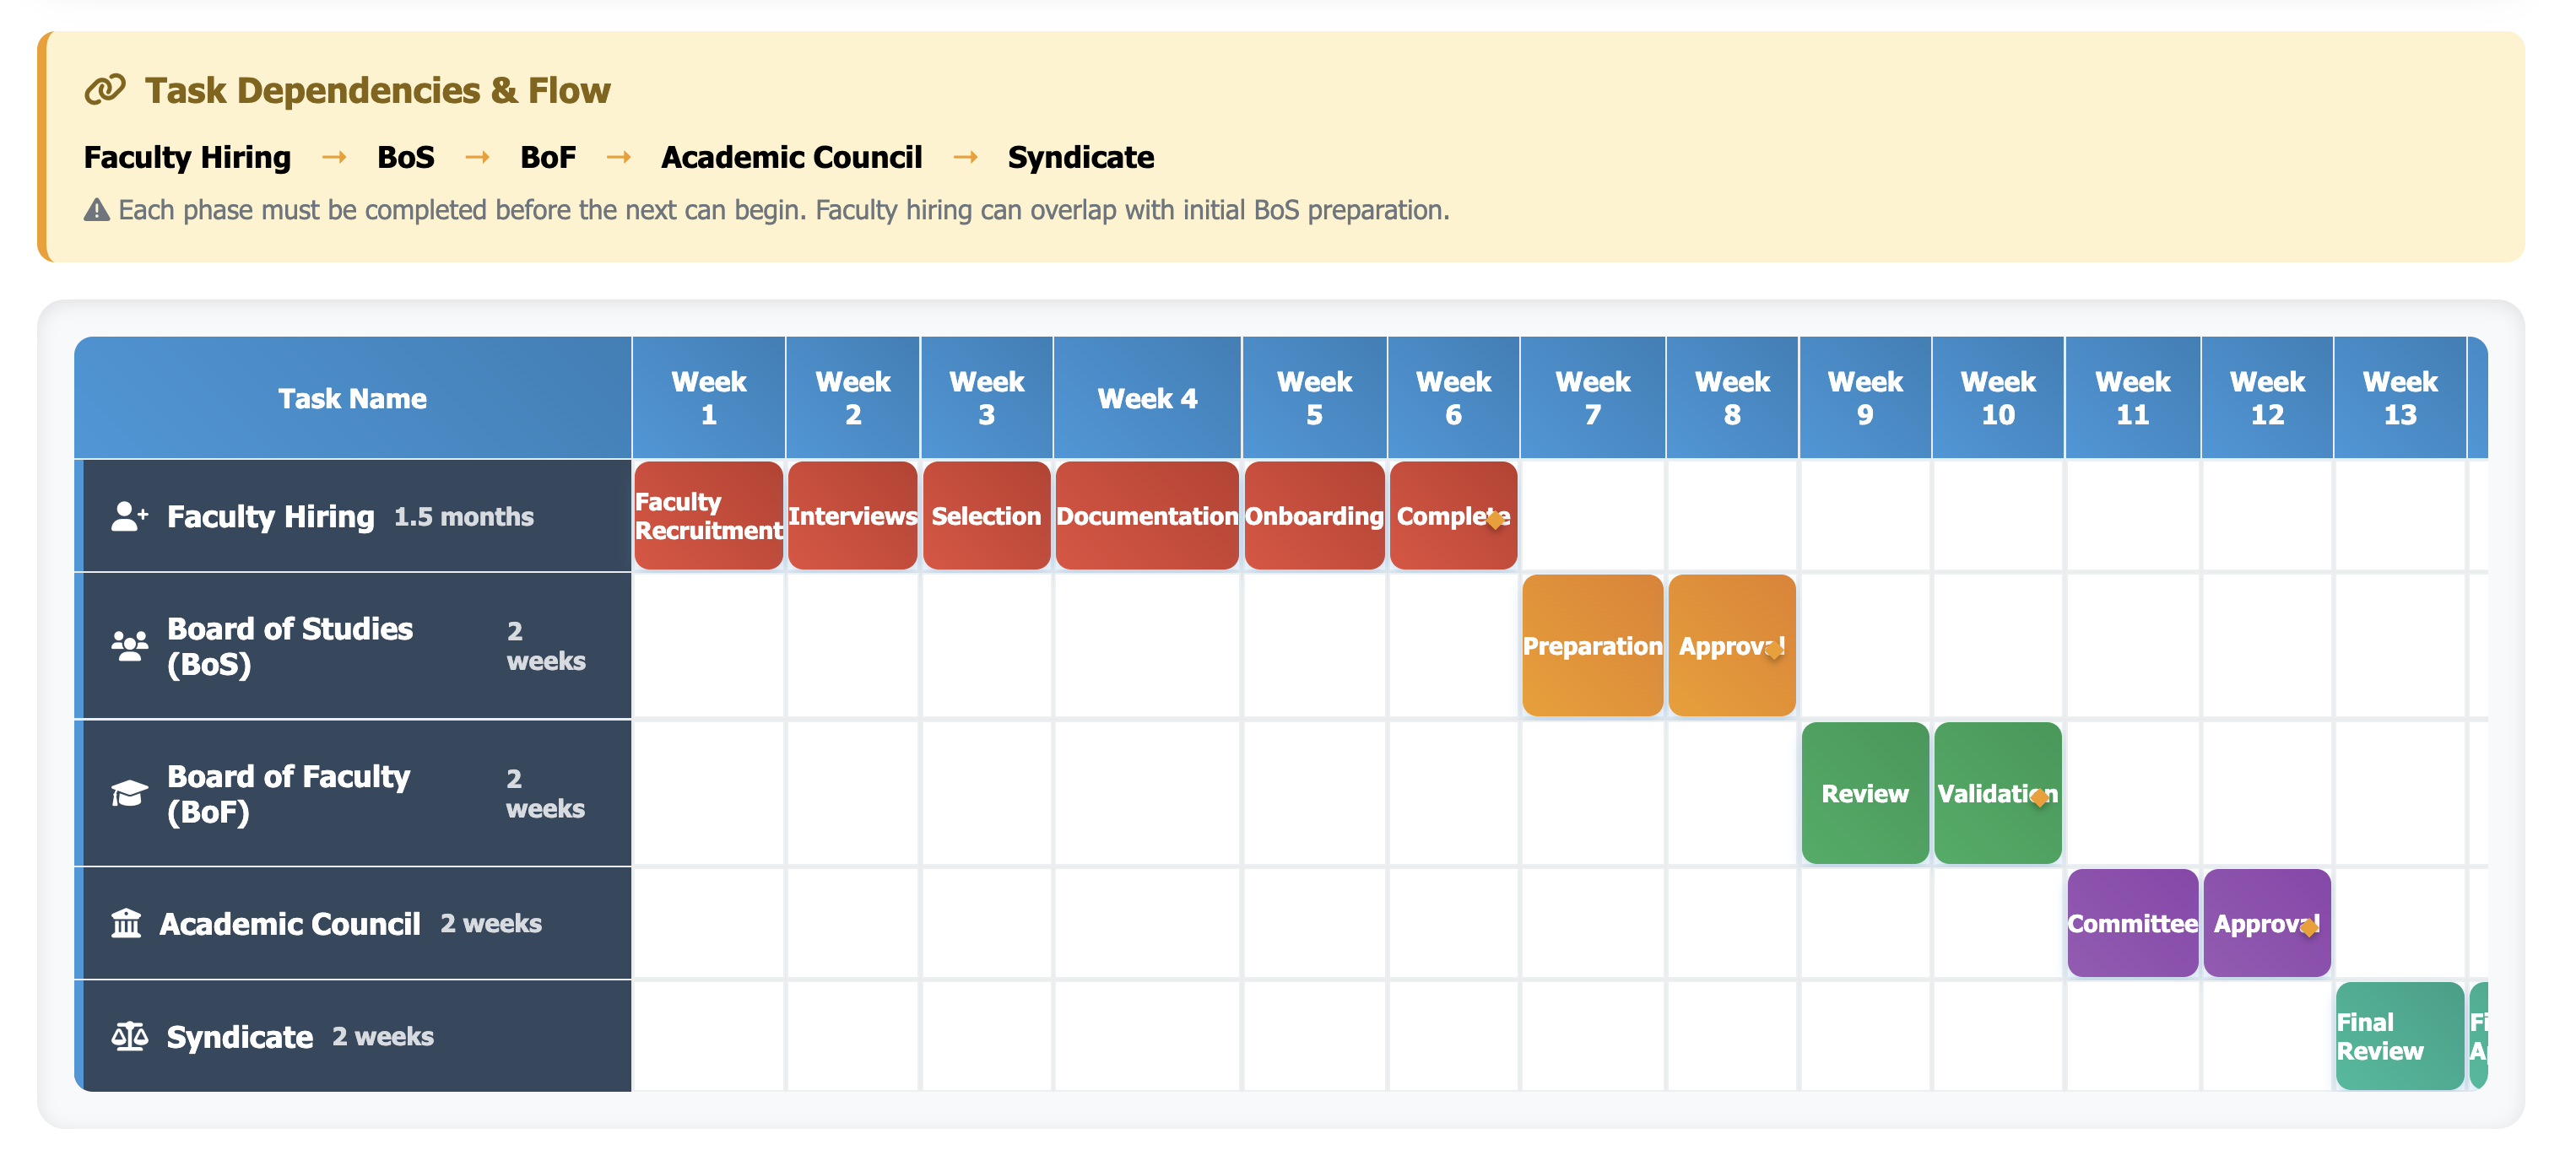
\includegraphics[width=0.5\textwidth]{/Users/TAYAB/Desktop/latexPractice/gain_chart.png}
%     \caption{Fig: Giant Chart for Demo}

% \end{figure}
% \end{document}

% =================== Lesson 6: Mathematical Equations ===================
% \documentclass{article}
% \usepackage{amsmath}

% \begin{document}

% \section{Simple Maths Equation}

% \subsection{Math Equation without using Package}
% Inline math: $E = mc^2$

% \textbf{Display Equation:}
% \begin{equation}
%     \sum_{i=1}^{n} x_i = x_1 + x_2 + ... + x_n
% \end{equation}

% \end{document}

% =================== Lesson 5: Lists ===================
% \documentclass{article}

% \begin{document}

% \section{My Lists}

% \subsection{Number List:}
% \begin{enumerate}
%     \item Flutter
%     \item Firebase
%     \item SQL Databases
% \end{enumerate}

% \subsection{Bullted List:}
% \begin{itemize}
%     \item Provider
%     \item MVVM
%     \item GetX
% \end{itemize}

% \end{document}

% =================== Lesson 4: Adding Title and Author =================== 
% \documentclass{article}

% \title{Intro To Mobile App Development using AI Agent Outperfrom than Human Development}
% \author{Tayab Farooq Khattak}
% \date{\today}
% \begin{document}

% \maketitle

% \end{document}

% =================== Lesson 3: Creating Sections =================== 
% \documentclass{article}

% \begin{document}

% \section{Introduction}
% Into Mobile App Development using Flutter

% \subsection{Background}
% You must know the basics of Programming. it is plus in case you know about Dart
% Programming Language

% \subsubsection{Tools Requirements}
% VS Code, Xcode, and PC with good specifications

% \end{document}

% =================== Lesson 2: Adding Text Formatting ===================
% \documentclass{article}
% \begin{document}

% This is a bit about text formating with \textbf{Bold Text} and now we have
% \textit{Italic Text}

% \end{document}

% =================== Lesson-1-Create super simple Doc ===================
% \documentclass{report}

% \begin{document}
% This is my first super simple document PDF file
% \end{document}

